\section{Base de données}
\label{sec:BD}


\subsection{Création de la base de données}
\label{sec:creation-db}

La base de données est composée de trois tables contenant toutes les données utiles au bon fonctionnement du site.\\
Il y a la table \textbf{Users} \textit{pour tout ce qui concerne les utilisateurs}, la table \textbf{Medicines}, \textit{qui concerne les médicaments} et le table \textbf{Reserves} \textit{qui contient la réserve de chaque utilisateur}.

\begin{figure}[h]
  \centering
  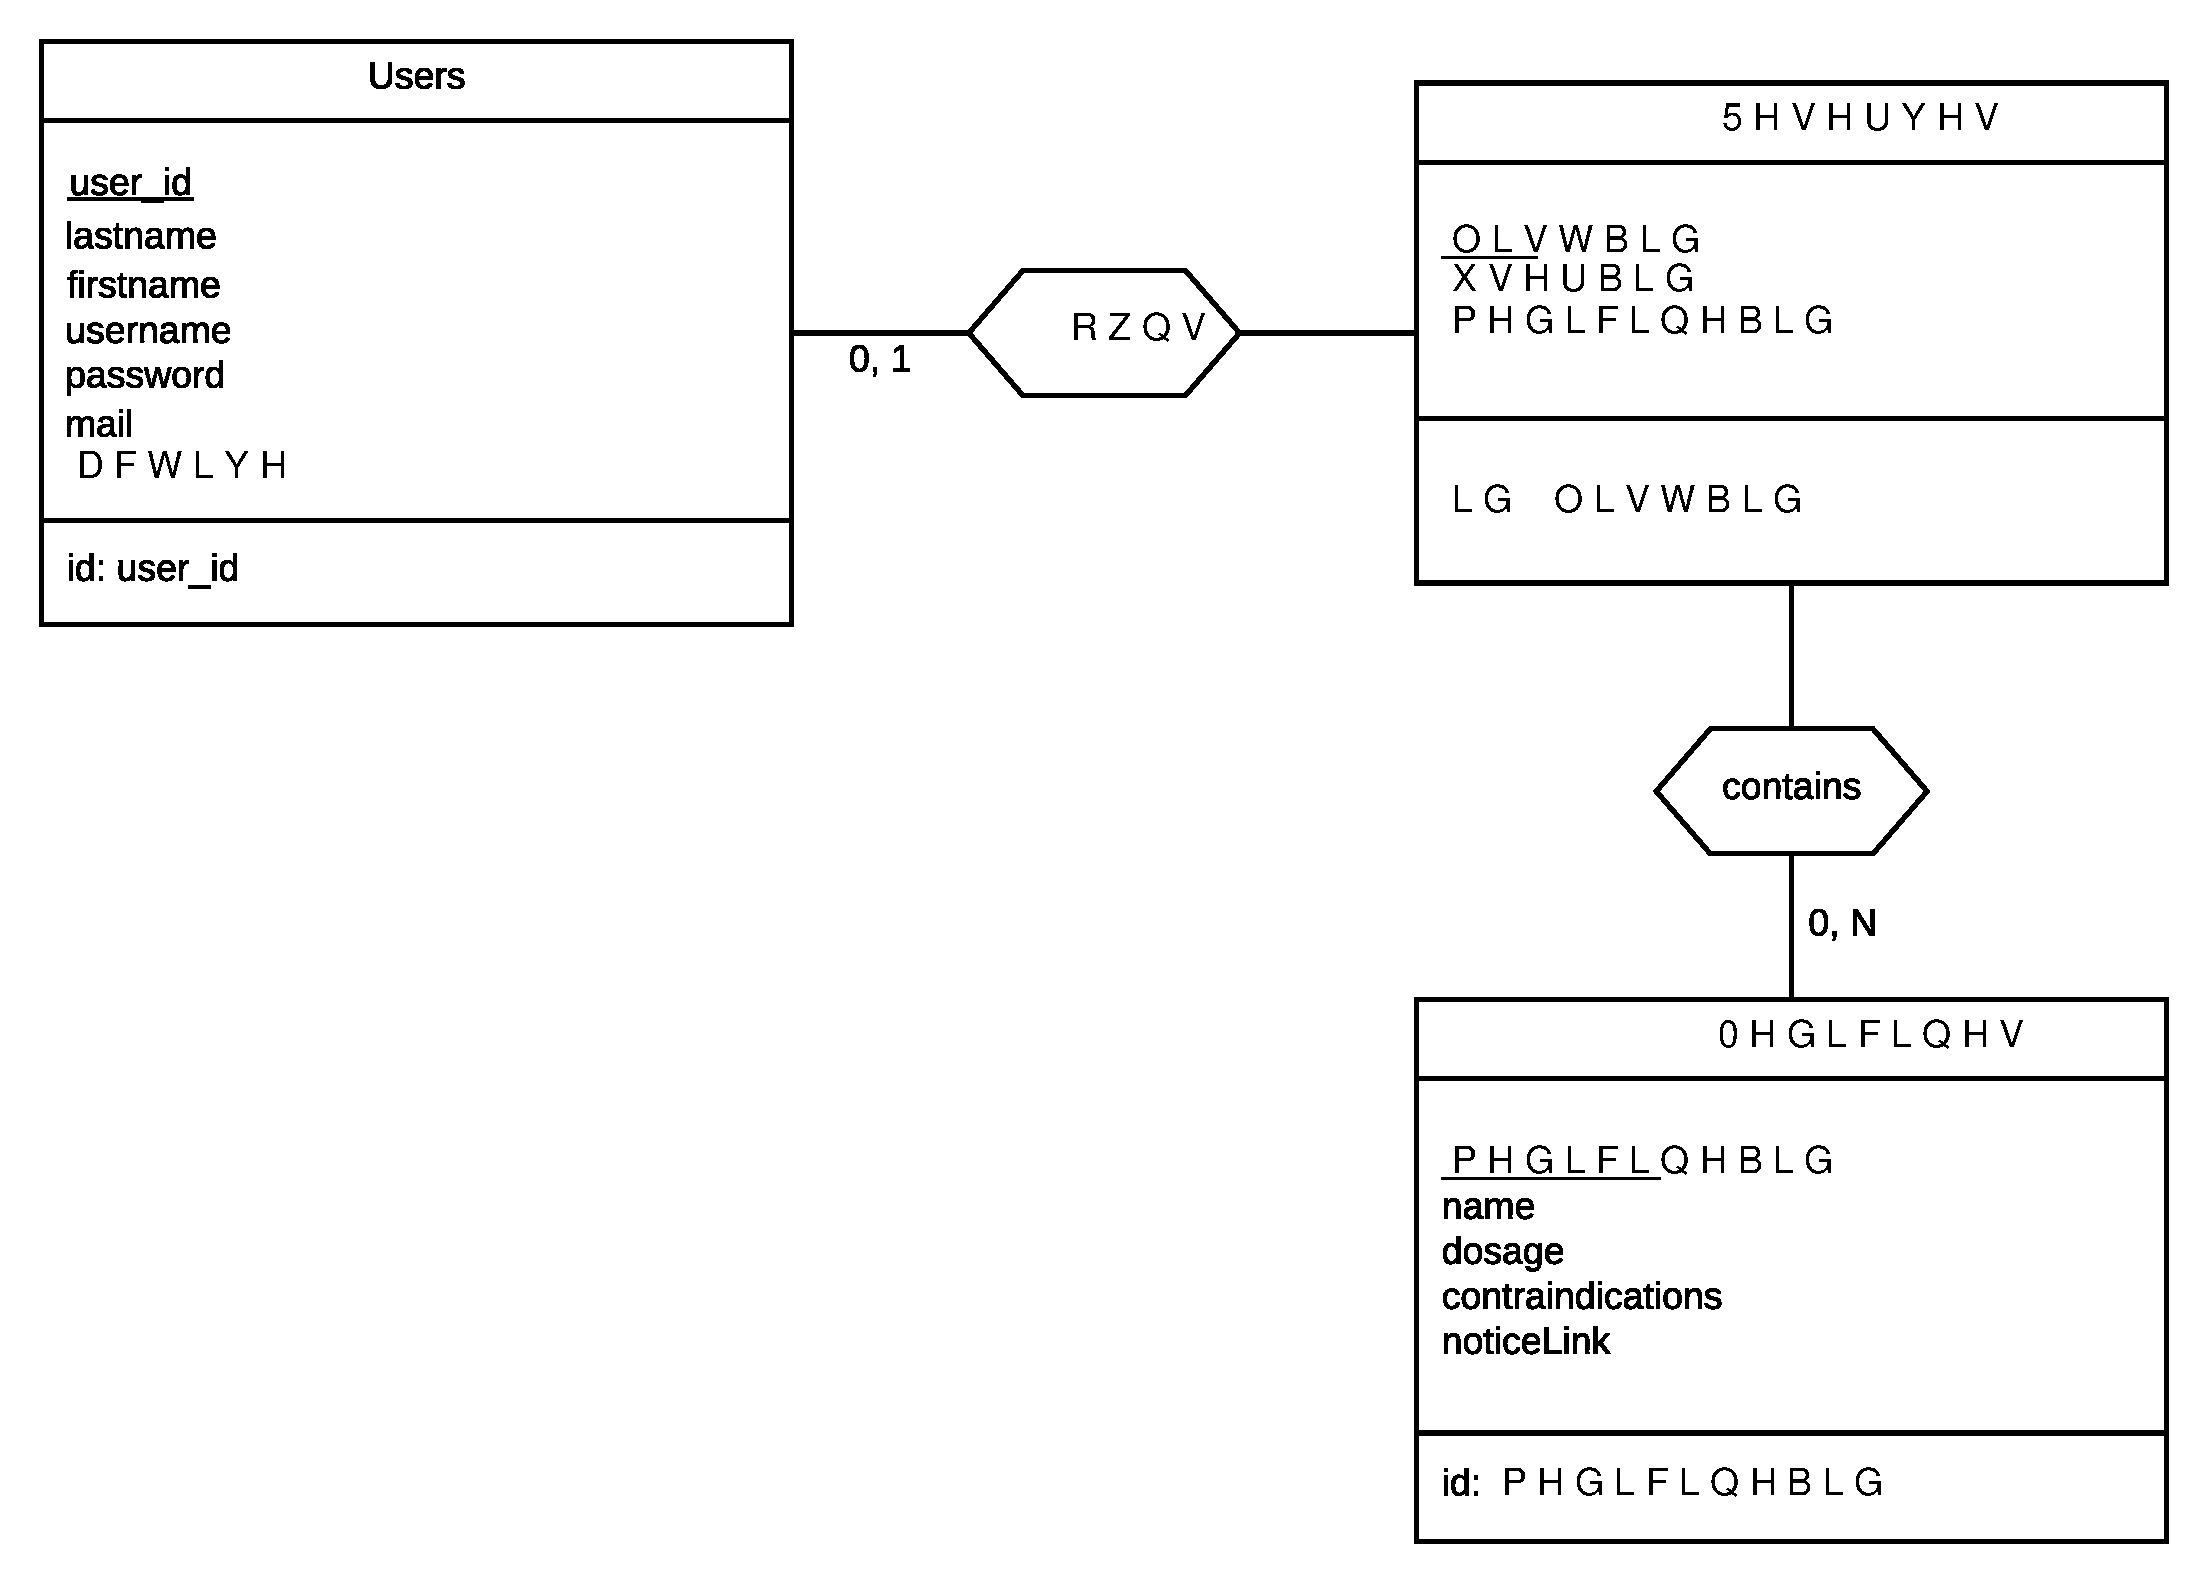
\includegraphics[scale=0.4]
  {textures/images/db/DB.pdf}
  \caption{Schéma conceptuel de la base de données}
  \label{fig:db}
\end{figure}

\newpage

\subsection{Vue détaillée}
\label{sec:vue-details}


\subsubsection{Table Medicines}
\label{sec:table-med}

Cette table contient les informations de chaque médicament.\\

\begin{itemize}
    
    \item[$\bullet$] \textbf{medicine\_id} est l'identifiant du médicament.\\
    Il sert de clé primaire de la table et est auto-incrémenté à partir de 1.
    
    \item[$\bullet$] \textbf{name} est le nom du médicament.\\
    Ce champ, en plus de contenir le médicament, identifie son type: comprimé, comprimé effervescent, gélule, etc.
    
    \item[$\bullet$] \textbf{dosage} contient le ou les différents dosages possibles \textit{(en mg ou en g)}.
    
    \item[$\bullet$] \textbf{contraindications} comprend deux à trois lignes de contre-indications du médicament.
    
    \item[$\bullet$] \textbf{noticeLink} contient l'adresse vers la notice en ligne, à télécharger.
    
\end{itemize}

\textbf{\textit{Remarque : }} l'image représentant le médicament est sauvegardée dans un dossier spécifique et est liée à son identifiant.\\
Elle ne se trouve donc pas dans la base de données.


\subsubsection{Table Reserves}
\label{sec:table-res}

Cette table lie les deux autres: la réserve de médicaments lie chaque utilisateur à ses médicaments.\\

\begin{itemize}

    \item[$\bullet$] \textbf{list\_id} est l'identifiant unique de la réserve.\\
    Il est auto-incrémenté à partir de un et sert de clé primaire.
    
    \item[$\bullet$] \textbf{user\_id} est l'identifiant de l'utilisateur.\\
    C'est une clé étrangère.
    
    \item[$\bullet$] \textbf{medicine\_id} identifie les médicaments.\\
    C'est aussi une clé étrangère.
    
\end{itemize}

\newpage

\subsubsection{Table Users}
\label{sec:table-users}

C'est la table contenant les données de chaque utilisateur ainsi que l'état de leur compte.\\

\begin{itemize}
    
    \item[$\bullet$] \textbf{user\_id} est l'identifiant unique du médicament.\\
    Il sert de clé primaire de la table et est auto-incrémenté à partir de un.
    
    \item[$\bullet$] \textbf{lastname} est le nom de famille de l'utilisateur.
    
    \item[$\bullet$] \textbf{firstname} est le prénom de l'utilisateur.
    
    \item[$\bullet$] \textbf{username} est le nom d'utilisateur unique choisi lors de l'inscription.
    
    \item[$\bullet$] \textbf{password} est le mot de passe de l'utilisateur.\\
    Il a une taille minimale de 4 caractères et est haché \footnote{\url{https://fr.wikipedia.org/wiki/Fonction\_de\_hachage\_cryptographique}} \textit{(et salé)} à l'aide de SHA512.
    
    \item[$\bullet$] \textbf{mail} contient l'adresse mail de l'utilisateur.\\
    Ce champ est unique, vu qu'il sert à la connexion de l'utilisateur.
    
    \item[$\bullet$] \textbf{active} donne l'état du compte de l'utilisateur:
    
    \begin{itemize}
        
        \item \textbf{0} indique que le compte est inactif.\\
        Cela signifie que le compte a été supprimé ou que l'administrateur a banni l'utilisateur.
        
        \item \textbf{1} indique que le compte est actif \textit{(par défaut)}.
        
    \end{itemize}
    
\end{itemize}


%%% Local Variables:
%%% mode: latex
%%% TeX-master: t
%%% End: